%!TeX encoding = UTF-8
%!TeX program = xelatex
\documentclass[
  notheorems,
  aspectratio=54,
]{beamer}

%% preamble
\title{Heavy–tailed neuronal connectivity arises from Hebbian self–organization}
% \subtitle{The subtitle}
\author{Jingsheng Gao}
\institute{Anqing Normal University}

\useoutertheme{shadow}
\setbeamertemplate{headline}{}
\mode<presentation>{
  \usetheme{Warsaw}
  \usecolortheme{seagull}
}

\setbeamertemplate{footline}
{
  \leavevmode%
  \hbox{%
  \begin{beamercolorbox}[wd=.57\paperwidth,ht=2.25ex,dp=1ex,center]{title in head/foot}%
    \usebeamerfont{title in head/foot}\inserttitle
  \end{beamercolorbox}%
  \begin{beamercolorbox}[wd=.33\paperwidth,ht=2.25ex,dp=1ex,center]{author in head/foot}%
      \usebeamerfont{author in head/foot}\insertauthor\ - \insertinstitute
  \end{beamercolorbox}%
  \begin{beamercolorbox}[wd=.1\paperwidth,ht=2.25ex,dp=1ex,right]{date in head/foot}%
    \insertframenumber{} / \inserttotalframenumber\hspace*{2ex} 
  \end{beamercolorbox}}%
  \vskip0pt%
}


\setbeamertemplate{navigation symbols}{}

\usepackage[
    backend=biber,
    autocite=superscript,
    sorting=none
]{biblatex}
\AtBeginBibliography{\small}
\addbibresource{refs.bib}

\usepackage{caption}
\captionsetup[figure]{font=scriptsize}

\usepackage{latexsym}
\usepackage{amsmath,amssymb}
\usepackage{mathtools}
\usepackage{color,xcolor}
\usepackage{graphicx}
\usepackage{algorithm}
\usepackage{amsthm}
\usepackage{lmodern}
% \usepackage[UTF8]{ctex}
% \usepackage{xeCJK}
\usepackage{animate} % insert gif

\usepackage{lipsum}
\usepackage{ulem}

\usepackage{listings} % display code on slides; don't forget [fragile] option after \begin{frame}

% ----------------------------------------------
% tikx
\usepackage{framed}
\usepackage{tikz}
\usepackage{pgf}
\usetikzlibrary{calc,trees,positioning,arrows,chains,shapes.geometric,%
    decorations.pathreplacing,decorations.pathmorphing,shapes,%
    matrix,shapes.symbols}



% ----------------------------------------------

% ---------------------------------------------------------------------
% Jet Black Theme
% \setbeamercolor{normal text}{fg=white,bg=black!90}
% \setbeamercolor{structure}{fg=white}
%
% \setbeamercolor{alerted text}{fg=red!85!black}
%
% \setbeamercolor{item projected}{use=item,fg=black,bg=item.fg!35}
%
% \setbeamercolor*{palette primary}{use=structure,fg=structure.fg}
% \setbeamercolor*{palette secondary}{use=structure,fg=structure.fg!95!black}
% \setbeamercolor*{palette tertiary}{use=structure,fg=structure.fg!90!black}
% \setbeamercolor*{palette quaternary}{use=structure,fg=structure.fg!95!black,bg=black!80}
%
% \setbeamercolor*{framesubtitle}{fg=white}
%
% \setbeamercolor*{block title}{parent=structure,bg=black!70!gray}
% \setbeamercolor*{block body}{fg=black,bg=black!10}
% \setbeamercolor*{block title alerted}{parent=alerted text,bg=black!15}
% \setbeamercolor*{block title example}{parent=example text,bg=black!15}
% ---------------------------------------------------------------------


% \newcommand{\reditem}[1]{\setbeamercolor{item}{fg=red}\item #1}

% \newcommand*{\Scale}[2][4]{\scalebox{#1}{\ensuremath{#2}}}

% -------------------------------------------------------------

% -------------------------------------------------------------

\begin{document}

% title frame
\begin{frame}
    \titlepage
\end{frame}

\begin{frame}{Introduction}
 \begin{itemize}
    \item A neural network is a group of interconnected units called neurons that send signals to one another.
    \item A biological neural network is a population of biological neurons chemically connected to each other by synapses.
    \item In networks of neurons, the connections are heavy–tailed, with a small number of neurons connected much more strongly than the vast majority of pairs.
    \item This paper proposes a minimal model of synaptic self–organization: connections are pruned at random, and the synaptic strength rearranges under a mixture of Hebbian and random dynamics.
  \end{itemize}
\end{frame}

\begin{frame}{1. Heavy–tailed neuronal connectivity}
  \begin{figure}
    \centering
  \end{figure}
  \begin{itemize}
    \item The partial connectome of the Drosophila central brain (Fig. 1a), with 14 million synapses linking over 21 thousand neurons.
    \item Despite the large number of synapses, 99\% of neuron pairs remain unconnected; and even among connected neurons, 50\% are only linked by a single synapse (Fig. 1b).
      \begin{figure}
        \begin{minipage}[b]{0.8\textwidth}
          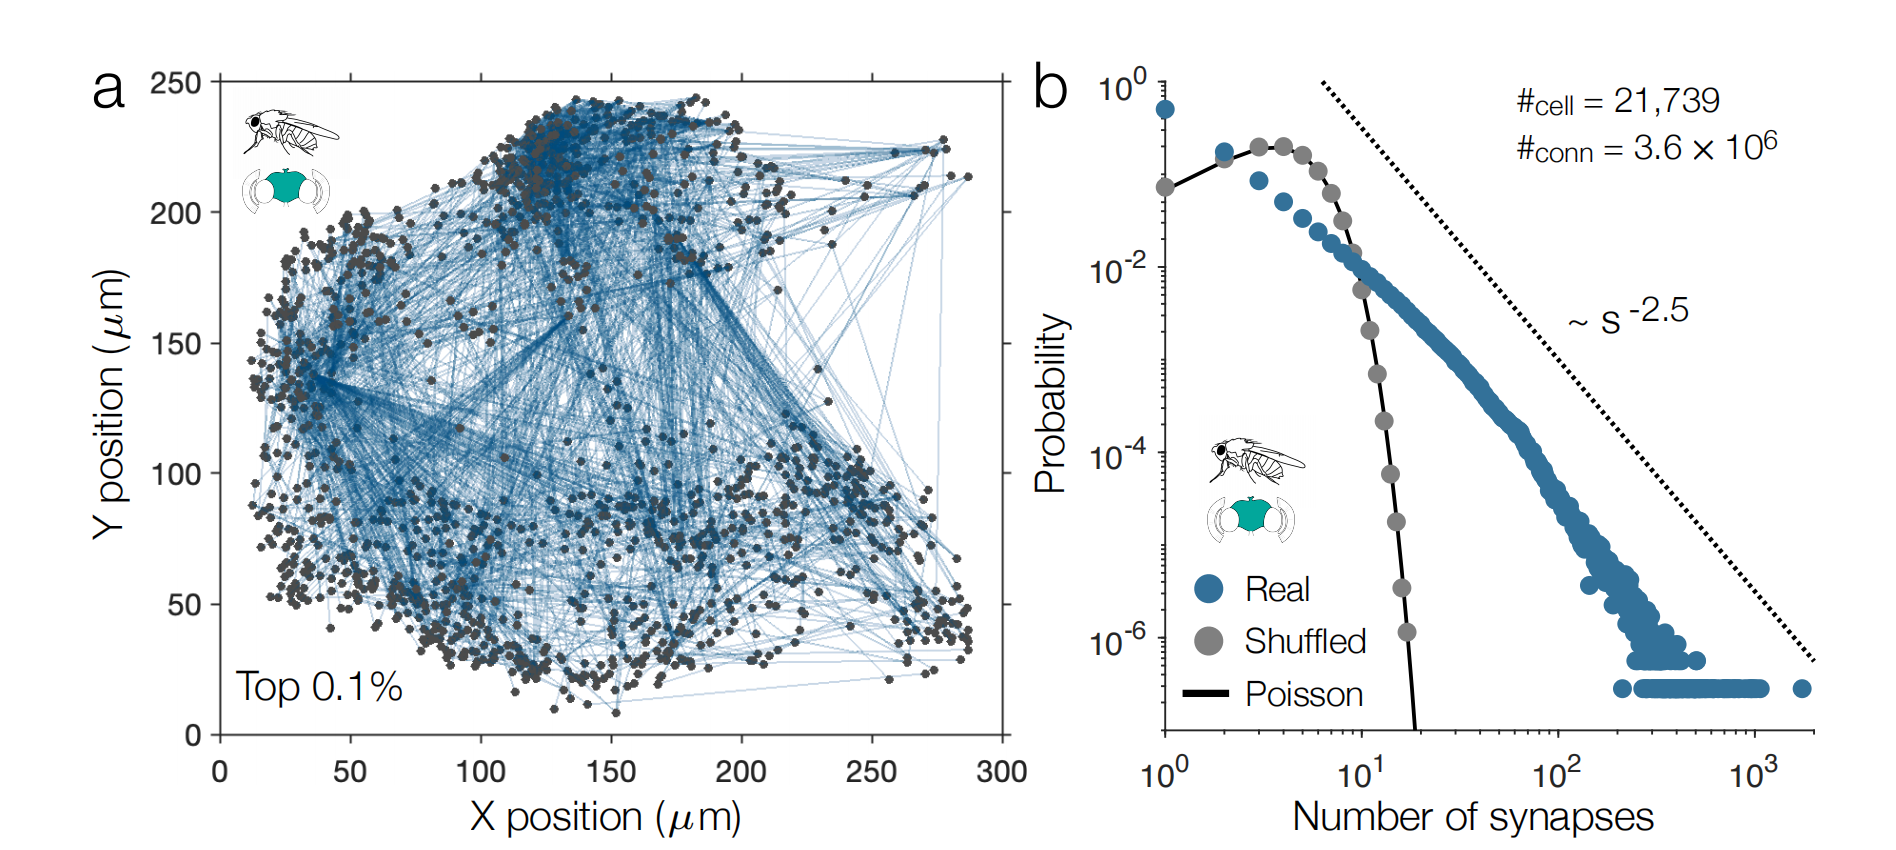
\includegraphics[width=0.8\textwidth]{Drosophila.png}
        \end{minipage}
      \end{figure}
    \item Meanwhile, some
pairs of neurons are connected by over one thousand individual synapses; these rare but extremely
strong connections comprise the heavy tail of synaptic connectivity (Fig. 1b).
  \end{itemize}
\end{frame}

\begin{frame}{1. Heavy–tailed neuronal connectivity}
  \begin{itemize}
   \item  Distributions of the number of
synapses in each connection of the Drosophila optic medulla (c), the entire connectome of the roundworm
C. elegans (d), and the sensory–motor circuit of the annelid Platynereis (e)
  \end{itemize}
  \begin{figure}
    \centering
    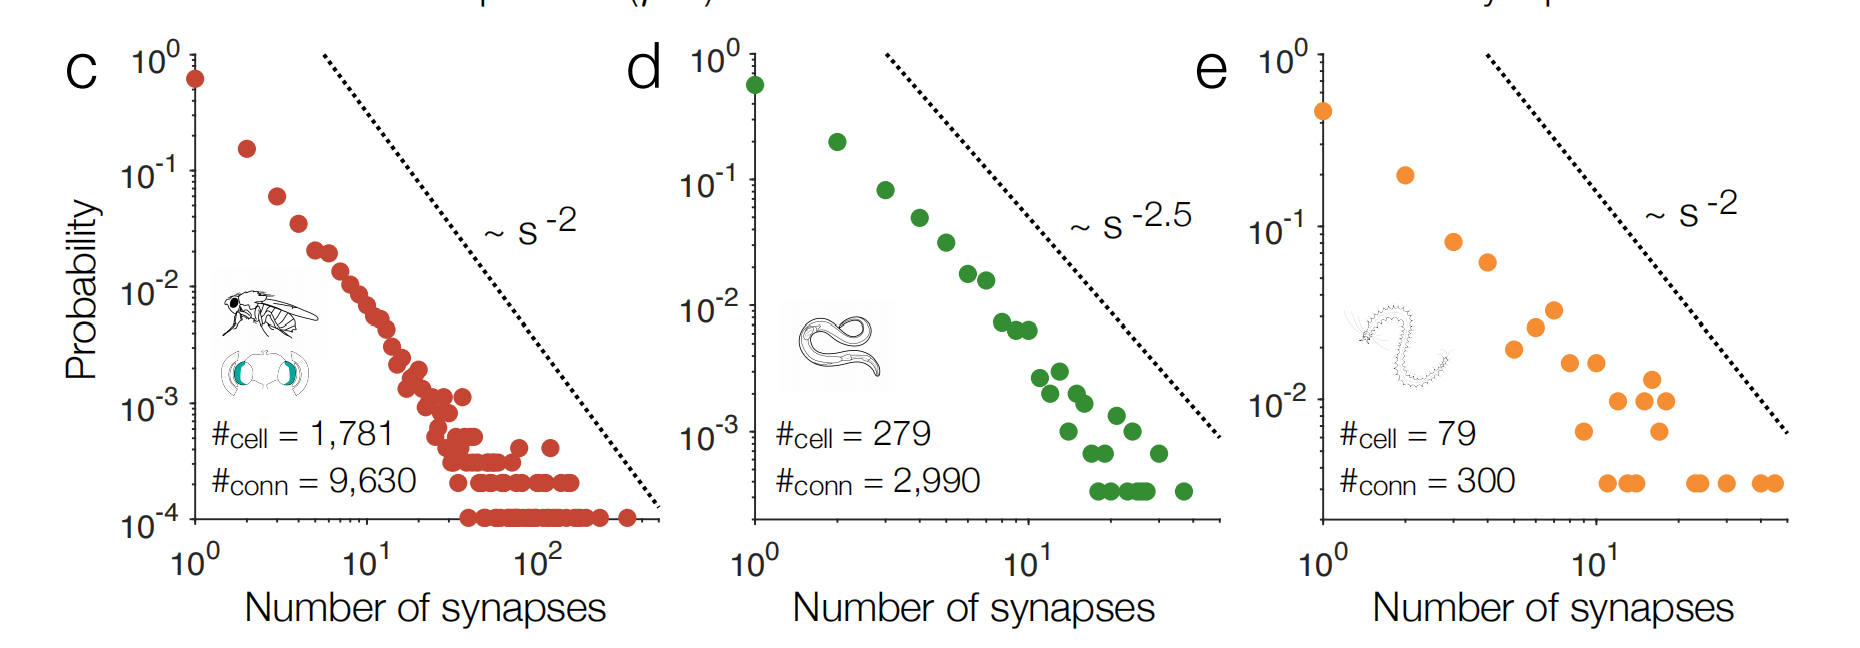
\includegraphics[width=0.8\textwidth]{./screenshot/3.png}
  \end{figure}
\end{frame}

\begin{frame}{1. Heavy–tailed neuronal connectivity}
  \begin{itemize}
    \item In invertebrates, stronger connections are formed by increasing the number of synapses in parallel.
    \item In vertebrates, connections are strengthened by increasing both the number and size of individual synapses.
    \item Distributions of the
number of contacts (f) and total contact area (g) between neurons in the inner plexiform layer of the mouse
retina. h, Distribution of covariances in neuronal activity in the mouse visual cortex while responding to
natural images, recorded using two–photon calcium imaging
  \end{itemize}
  \begin{figure}
    \centering
    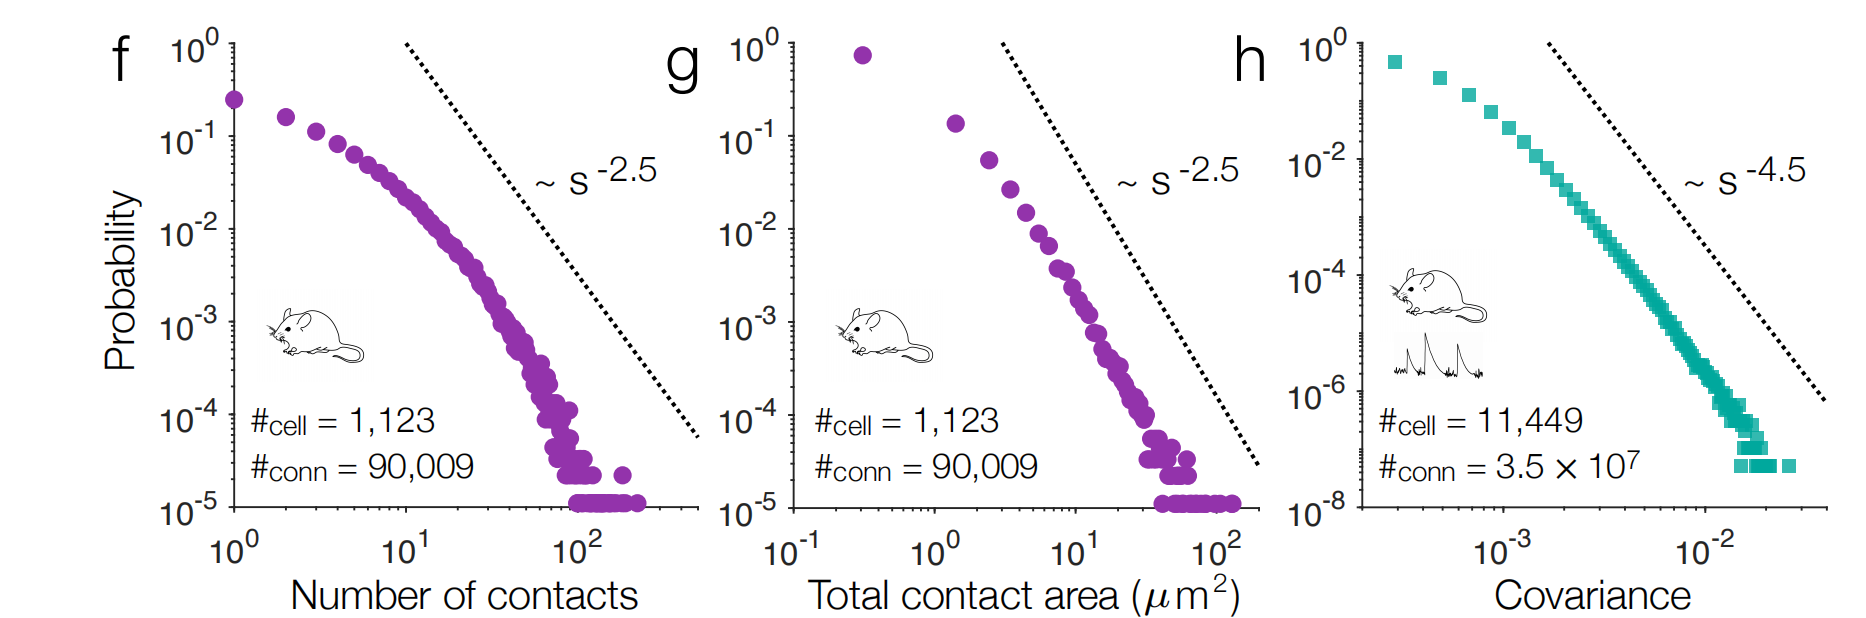
\includegraphics[width=0.8\textwidth]{./screenshot/4.png}
  \end{figure}
\end{frame}

\begin{frame}{2. Model of Hebbian self–organization}
  \begin{itemize}
    \item The above results suggest that heavy–tailed connectivity is a general feature of neuronal networks.
    \item In the study of complex systems, heavy-tailed distributions often arise from preferential attachment or rich–get–richer mechanisms.
    \item Hebbian plasticity, wherein strongly–connected neurons are more likely to cofire, leading to even further growth, is similar to the mechanisms mentioned above.
  \end{itemize}
\end{frame}

\begin{frame}{2. Model of Hebbian self–organization}
  \begin{itemize}
    \item Minimal model of Hebbian
network dynamics. At each time step, a random connection is pruned (left), and each unit of pruned strength
is redistributed either in a Hebbian fashion (with probability p; top) or randomly (with probability 1 −
p; bottom).
  \end{itemize}
  \begin{figure}
    \centering
    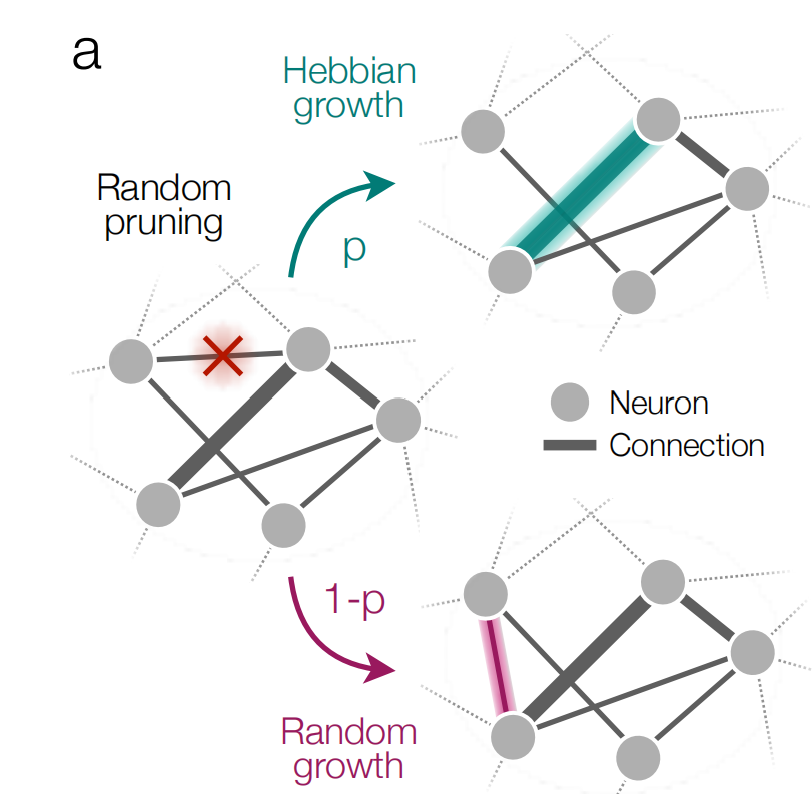
\includegraphics[width=0.6\textwidth]{./screenshot/5.png}
  \end{figure}
\end{frame}

\begin{frame}{2. Model of Hebbian self–organization}
  \begin{itemize}
    \item Analytic model predictions of the
Drosophila central brain (e),1 Drosophila optic medulla (f), C. elegans connectome (g), Platynereis
sensory–motor circuit (h), and mouse retina (i).
  \end{itemize}
  \begin{figure}
    \centering
    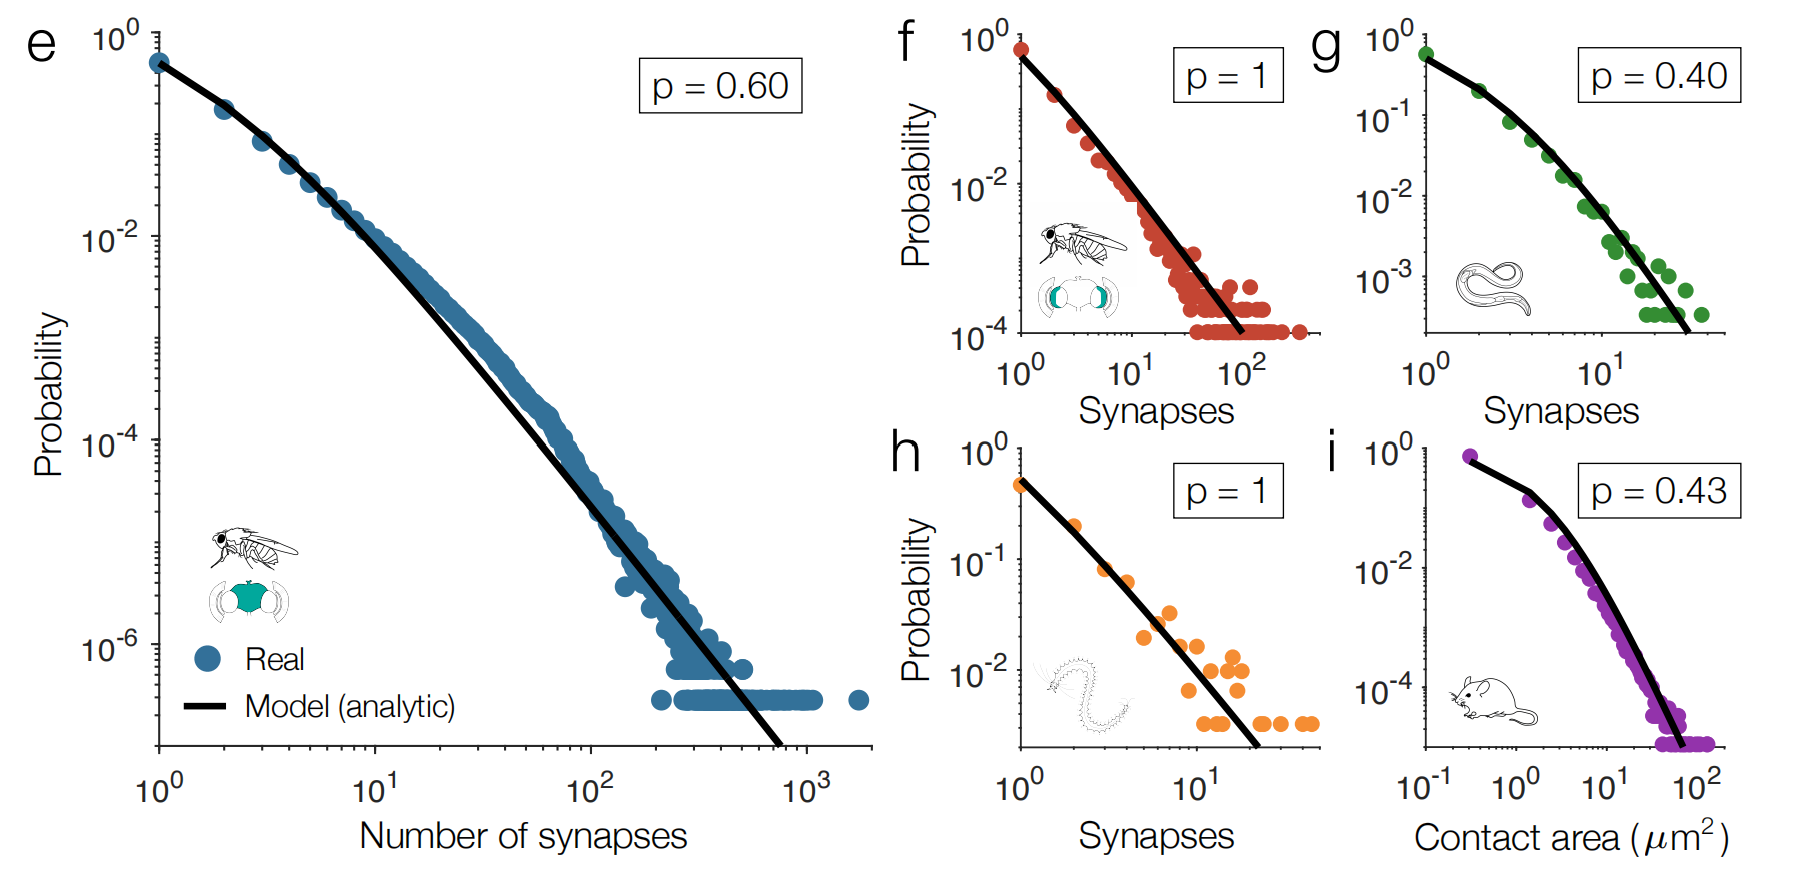
\includegraphics[width=0.8\textwidth]{./screenshot/7.png}
  \end{figure}
\end{frame}

\begin{frame}{3. Activity–dependent plasticity produces clustering}
  \begin{itemize}
    \item The model above generates networks with realistic connection strengths, even without including the effects of neuronal activity.
    \item In classical Hebbian plasticity, synaptic connections evolve not just on their own, but also in response to the correlations between neurons.
    \item Propose a model of neuronal activity to extend former network dynamics to include activity–dependent plasticity.
  \end{itemize}
\end{frame}

\begin{frame}{3.1 Model of neuronal activity}
  \begin{itemize}
    \item While
      one can implement varying degrees of biological realism, for simplicity here we consider artificial neurons that, between each network update, reach steady–state activities $x_{i}$ defined by
      the self–consistent equations $x_{i} = tanh(\beta\sum_{j}{A_{ij}x_{j}}) $
      , where $\beta \geq 0$ parameterizes the strength
      of interactions, and the connections $A_{ij}$ are implicitly normalized by $N\bar{s}$ (see Methods).
  \end{itemize}
\end{frame}

\begin{frame}{3.2 Activity–dependent plasticity}
  \begin{itemize}
    \item We are now prepared to extend our network dynamics to include activity–dependent plasticity. The random pruning and random growth remain unchanged;
      but for Hebbian growth, rather than selecting a connection with probability proportional to its current strength $A_{ij}$ , we instead select a pair of neurons with probability proportional to their covariance $C_{ij}$.
  \end{itemize}
  \begin{figure}
    \centering
    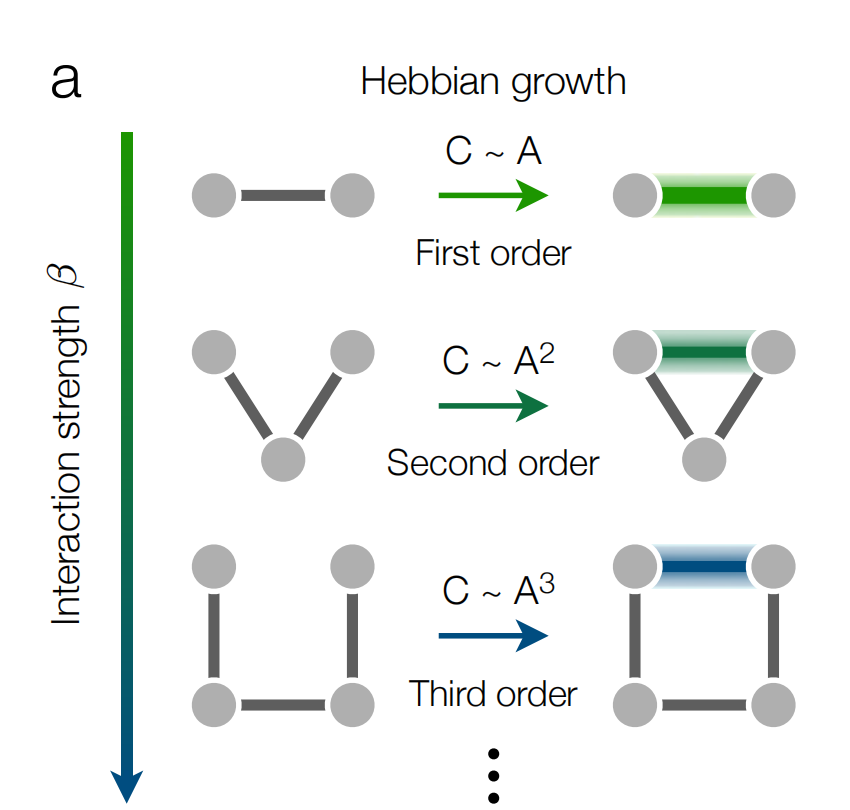
\includegraphics[width=0.5\textwidth]{./screenshot/8.png}
  \end{figure}
\end{frame}

\begin{frame}{3.2 Activity–dependent plasticity}
  \begin{itemize}
    \item Distributions of connection strengths for different interaction strengths interaction strength
      $\beta$ in networks of $N = 103$ neurons, Hebbian probability $p = 0.5$, and average connection strength $\bar{s} = 1$.
  \end{itemize}
  \begin{figure}
    \centering
    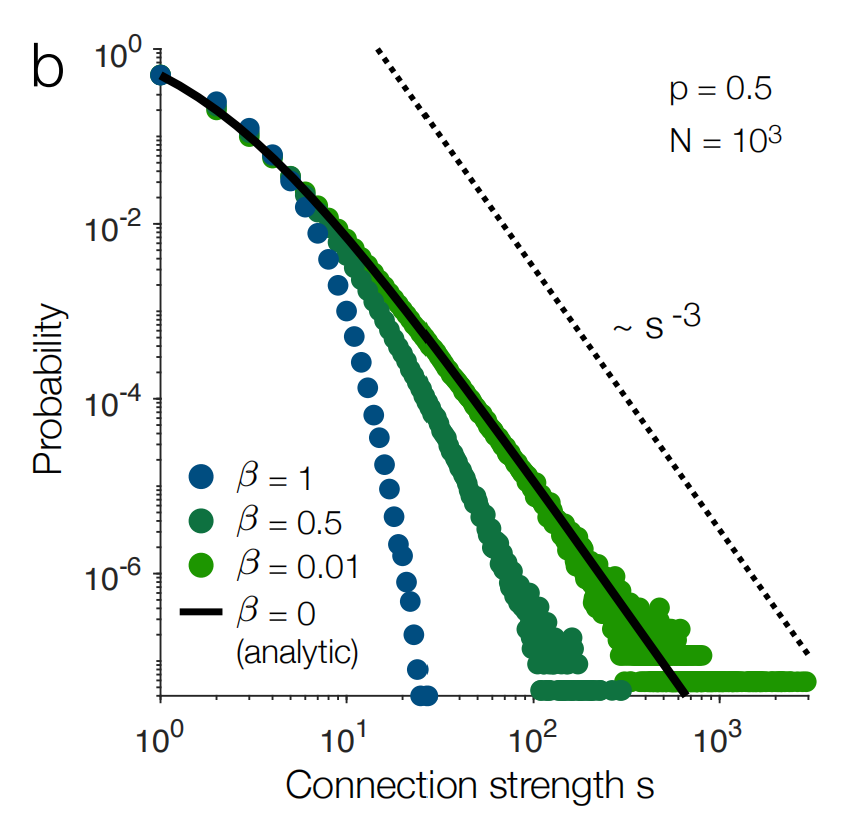
\includegraphics[width=0.5\textwidth]{./screenshot/9.png}
  \end{figure}
\end{frame}

\begin{frame}{3.3 Clustering}
  \begin{itemize}
    \item Real neuronal networks are known to exhibit a high density of triangles, a property known as clustering.
    \item Clustering is typically quantified using the ratio $N_{\triangle}/N_{\wedge}$ of the number of neuron triangles $N_{\triangle}$ to the
number of triplets $N_{\wedge}$ (sets of three neurons with at least two connections).
  \end{itemize}
\end{frame}

\begin{frame}{3.3 Clustering}
  \begin{itemize}
    \item Simulating
      networks with the same average connection strength $\bar{s}$ as the Drosophila central brain, the original
activity–independent model can capture the connection heterogeneity observed in the data, but fails to produce realistic clustering (Fig. b). However,
by generalizing to activity–dependent plasticity, the networks can simultaneously attain both the
connection heterogeneity and clustering observed in the Drosophila connectome (Fig. c)
  \end{itemize}
  \begin{figure}
    \centering
    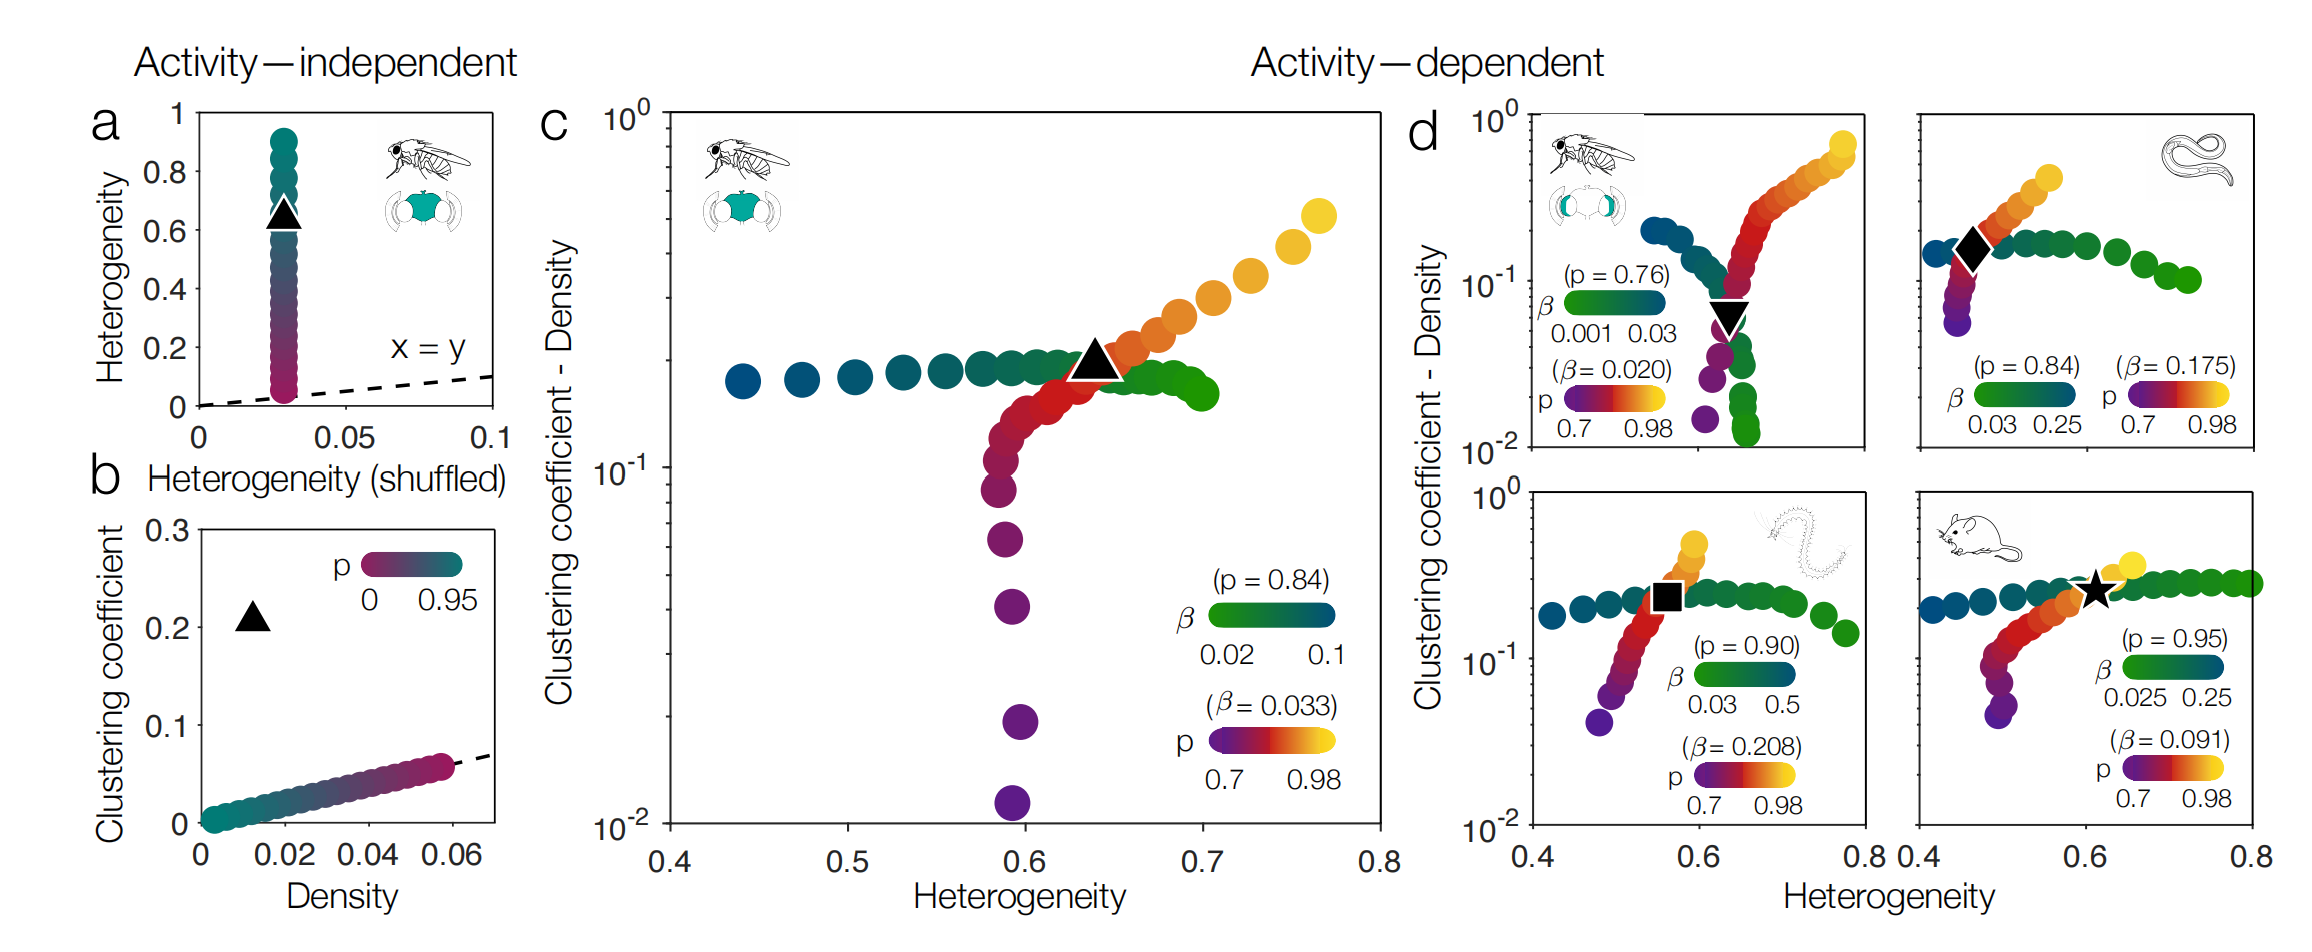
\includegraphics[width=0.8\textwidth]{./screenshot/10.png}
  \end{figure}
\end{frame}

\begin{frame}{4 Conclusion}
  \begin{itemize}
    \item Across a diverse range of species, the strengths of neuronal connections are similarly heavy–tailed, suggesting a common underlying mechanism. Here, we develop a minimal model
in which synaptic connectivity self–organizes under a mixture of Hebbian and random dynamics.
    \item Moreover, by
generalizing the model to include activity–dependent plasticity, the network dynamics naturally
give rise to clustering, another prominent feature of neuronal connectivity.
    \item Given
the simplicity of the model, future work can immediately begin to include more realistic plasticity
mechanisms, which, in turn, may produce additional properties observed in neuronal connectomes.
  \end{itemize}
\end{frame}


\nocite{*}
\begin{frame}{References}
    \printbibliography
\end{frame}

\begin{frame}{}
  \centering \Huge
  \emph{Thanks for listening!}
\end{frame}

\end{document}



